\documentclass[language = czech]{webquiz}

\BreadCrumbs{Matematika https://www.math.muni.cz/\string~xvasicekm | Kombinatorika https://www.math.muni.cz/\string~xvasicekm/kombiIndex.html | title}

\title{Základní kombinatorická pravidla}

\usepackage[czech]{babel}
\usepackage{hyperref}
\usepackage[dvipdfmx]{graphicx}

\begin{document}

	\begin{discussion}[Pravidlo součtu]\label{d1} %Prometheus 
		 Jsou-li $A_1,A_2,\dots,A_n$ konečné množiny, které mají po řadě $p_1,p_2,\dots,p_n$ prvků a jsou-li každé dvě disjunktní, pak počet prvků množiny $A_1 \cap A_2 \cap \dots \cap A_n$ je roven $p_1 + p_2 + \dots + p_n$.\\ Pokud potřebujete podrobnější vysvětlení, najdete ho \href{https://www.youtube.com/watch?v=kVWRTzAdc-U}{zde}.
	\end{discussion}
	
	\begin{discussion}[Pravidlo součinu]\label{d2} %Prometheus
		 Počet všech uspořádaných $k$-tic, jejichž první člen lze vybrat $n_1$ způsoby, druhý člen po výběru prvního členu $n_2$ způsoby atd. až $k$-tý člen po výběru všech předcházejících členů $n_k$ způsoby, je roven $n_1\cdot n_2 \cdot \dots \cdot n_k$.\\ Pokud potřebujete podrobnější vysvětlení, najdete ho \href{https://www.youtube.com/watch?v=JLheSkk4yWQ}{zde}.
	\end{discussion}
	
	\begin{question} \label{o1} %7.1-7/76
		Ze 120 studentů v ročníku ovládá 55 studentů angličtinu, 34 němčinu a 26 oba jazyky. Kolik studentů neovládá žádný z obou jazyků?
		\answer[integer]{57}
		\whenRight Jen tak \qref[dál]{o2}
		\whenWrong Zkus si nakreslit \href{https://www.youtube.com/watch?v=5c_m2EA0sN8}{vennovy diagramy}.
	\end{question}
	
	\begin{question} \label{o2} %7.1-9/76
		V autoopravně odstranili za jeden den na 46 automobilech 36 poruch motorů a 24 poruch brzd. Přitom na každém z opravovaných aut nebylo více oprav stejného druhu. Kolik aut mělo pouze poruchu motoru a kolik jich mělo jen poruchu na brzdách?
		\begin{choice}[columns=3]
			\incorrect Poruch jen motorů: 10, jen brzd: 22
				\feedback Dej pozor na prohození poruch motorů za poruchy brzd.
			\incorrect Poruch jen motorů: 14, jen brzd: 24
				\feedback Zkus si nakreslit \href{https://www.youtube.com/watch?v=5c_m2EA0sN8}{vennovy diagramy} a uvědomit si, kolik aut mělo zároveň poruchu motoru i brzd.
			\correct Poruch jen motorů: 22, jen brzd: 10
				\feedback Dobrá práce \qref[další otázka]{o3} už čeká
			\incorrect Poruch jen motorů: 26, jen brzd: 14
				\feedback kus si nakreslit \href{https://www.youtube.com/watch?v=5c_m2EA0sN8}{vennovy diagramy} a uvědomit si, kolik aut mělo zároveň poruchu motoru i brzd.
			\incorrect Poruch jen motorů: 22, jen brzd: 24
				\feedback Potom by žádné auto nemělo obě poruchy zároveň, zkus si nakreslit \href{https://www.youtube.com/watch?v=5c_m2EA0sN8}{vennovy diagramy} a uvědomit si, kolik aut mělo zároveň poruchu motoru i brzd. 
			\incorrect Poruch jen motorů: 36, jen brzd: 10
				\feedback Potom by žádné auto nemělo obě poruchy zároveň, zkus si nakreslit \href{https://www.youtube.com/watch?v=5c_m2EA0sN8}{vennovy diagramy} a uvědomit si, kolik aut mělo zároveň poruchu motoru i brzd. 
		\end{choice}	
	\end{question}
	
	\begin{question} \label{o3} %7.1-6a)/76
		Je známo, že jeden volitelný předmět navštěvuje 30 studentů a druhý 24 studentů. Co z těchto údajů vyplývá pro celkový počet studentů navštěvujících oba předměty, jestliže se konají v různé době s účastí týchž 15 studentů?
		\answer[integer]{39}
		\whenRight Jen tak \qref[dál]{o4}, možná se ti ale bude hodit podívat se na \dref[pravidlo součinu]{d2}.
		\whenWrong Označme: $A$ množinu všech studentů navštěvující 1. předmět ($|A|=30$), $B$ množinu studentů navštěvujících 2.předmět ($|B|=24$). Protože $A\cap B \neq \emptyset$ ($|A\cap B| = 15$), pak podle $|A\cup B| = |A| + |B| - |A\cap B|$. A tedy všech studentů ($|A\cup B|$) je$\dots$ Zkus další pokus :).\\ Pro znázornění můžeš použít \href{https://www.youtube.com/watch?v=5c_m2EA0sN8}{vennovy diagramy}.
	\end{question}
	
	\begin{question} \label{o4} %7.1-15a)/76
		Určete, kolik je všech dvojciferných přirozených čísel.\\ \textit{Nápověda: použijte} \dref[pravidlo součinu]{d2}
		\answer[integer]{90}
		\whenRight Vypadá to, že pravidlo součinu začínáš ovládat. Zkus \qref[další otázku]{o5}.
		\whenWrong Na vytváření dvojciferných čísel se můžeme podívat tak, že máme dvě volné pozice ( \_ \_ ). Máme deset cifer \{0,1,2,\dots ,8,9\}. Na první pozici můžeme dosadit 9 z nich, protože dvojciferné číslo nesmí začínat nulou. Na druhou pozici můžeme dosadit libovolnou cifru. Podle pravidla součinu, potom $9\cdot 10$ je počet všech možností.
	\end{question}
	
	\begin{question} \label{o5} %7.1-18/77
		Do studentské samosprávy je třeba zvolit jednoho zástupce z každé ze dvou tříd, v nichž je 28 a 30 studentů. Kolika různými způsoby lze tuto volbu provést?
		\answer[integer]{840}
		\whenRight Dobrá práce, \qref[další otázka]{o6} se na tebe těší.
		\whenWrong Uvědom si, kolik studentů můžeš zvolit z první třídy a kolik studentů ze třídy druhé. Potom zkus aplikovat \dref[pravidlo součinu]{d2}.
	\end{question}
	
	\begin{question} \label{o6} %7.1-19/77
		Z 12 různých košil, 9 různých kravat a 11 různých párů ponožek se má vybrat jedno oblečení. Kolika různými způsoby se může tento výběr provést?
		\answer[integer]{1188}
		\whenRight Pravidlo součinu už očividně ovládáš. \qref[Dál]{o7}.
		\whenWrong Uvědom si, kolika způsoby můžeš zvolit košili, kolika kravatu a kolika ponožky. Potom zkus aplikovat \dref[pravidlo součinu]{d2}.
	\end{question}
	
	\begin{question} \label{o7} %7.1-20/77
		Máme k dispozici 12 červených, 15 bílých a 8 žlutých růží, 25 červených, 14 bílých a 18 dvoubarevných karafiátů. Kolik různých kytic obsahujících právě tři různé růže nebo právě tři různé karafiáty lze z nich udělat?
		\answer[integer]{7740}
		\whenRight Dobrá práce, už máš skoro hotovo. \qref[poslední otázka]{o8}.
		\whenWrong Je potřeba si uvědomit, že pomocí \dref[pravidla součinu]{d2} zjistíme počet možných vytvořených kytic růží a kolik kytic karafiátů. Na tyto počty možností poté aplikujeme \dref[pravidlo součtu]{d1}. 
	\end{question}
	
	\begin{question} \label{o8} %7.1-21e)/77
		Z místa $M_1$ do místa $M_2$ vedou cesty $a, b, c, d$ a z místa $M_2$ do místa $M_3$ vedou cesty $e, f$.\\
		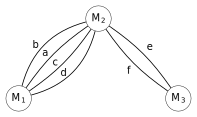
\includegraphics[scale=2]{701-21.svg}\\
		 Určete počty všech cestovních tras, tj. způsobů, jimiž se lze dostat po trase z místa $M_1$ do místa $M_3$ a zpět tak, že přitom projde místem $M_2$ právě dvakrát za podmínky, že právě jedna z šesti cest je použita dvakrát.
		\answer[integer]{32}
		\whenRight Paráda! Už máš hotovo :).
		\whenWrong Musíš opět použít \dref[pravidla součinu]{d2} i \dref[pravidlo součtu]{d1}.
	\end{question}
	
\end{document}

























